% !TeX spellcheck = en_GB
% THIS IS SIGPROC-SP.TEX - VERSION 3.1
% WORKS WITH V3.2SP OF ACM_PROC_ARTICLE-SP.CLS
% APRIL 2009
%
% It is an example file showing how to use the 'acm_proc_article-sp.cls' V3.2SP
% LaTeX2e document class file for Conference Proceedings submissions.
% ----------------------------------------------------------------------------------------------------------------
% This .tex file (and associated .cls V3.2SP) *DOES NOT* produce:
%       1) The Permission Statement
%       2) The Conference (location) Info information
%       3) The Copyright Line with ACM data
%       4) Page numbering
% ---------------------------------------------------------------------------------------------------------------
% It is an example which *does* use the .bib file (from which the .bbl file
% is produced).
% REMEMBER HOWEVER: After having produced the .bbl file,
% and prior to final submission,
% you need to 'insert'  your .bbl file into your source .tex file so as to provide
% ONE 'self-contained' source file.
%
% Questions regarding SIGS should be sent to
% Adrienne Griscti ---> griscti@acm.org
%
% Questions/suggestions regarding the guidelines, .tex and .cls files, etc. to
% Gerald Murray ---> murray@hq.acm.org
%
% For tracking purposes - this is V3.1SP - APRIL 2009

\documentclass{acm_proc_article-sp-copy}

\begin{document}
	
\title{Automatically Deploy Deep Learning Models on FPGA}
%\title{F-TensorFlow: Automatically Deploying TensorFlow Described Deep Learning Models on FPGA with High Performance}

%\subtitle{[Extended Abstract]
%\titlenote{A full version of this paper is available as
%\textit{Author's Guide to Preparing ACM SIG Proceedings Using
%\LaTeX$2_\epsilon$\ and BibTeX} at
%\texttt{www.acm.org/eaddress.htm}}}
%
% You need the command \numberofauthors to handle the 'placement
% and alignment' of the authors beneath the title.
%
% For aesthetic reasons, we recommend 'three authors at a time'
% i.e. three 'name/affiliation blocks' be placed beneath the title.
%
% NOTE: You are NOT restricted in how many 'rows' of
% "name/affiliations" may appear. We just ask that you restrict
% the number of 'columns' to three.
%
% Because of the available 'opening page real-estate'
% we ask you to refrain from putting more than six authors
% (two rows with three columns) beneath the article title.
% More than six makes the first-page appear very cluttered indeed.
%
% Use the \alignauthor commands to handle the names
% and affiliations for an 'aesthetic maximum' of six authors.
% Add names, affiliations, addresses for
% the seventh etc. author(s) as the argument for the
% \additionalauthors command.
% These 'additional authors' will be output/set for you
% without further effort on your part as the last section in
% the body of your article BEFORE References or any Appendices.

%\numberofauthors{8} %  in this sample file, there are a *total*
% of EIGHT authors. SIX appear on the 'first-page' (for formatting
% reasons) and the remaining two appear in the \additionalauthors section.
%

% Just remember to make sure that the TOTAL number of authors
% is the number that will appear on the first page PLUS the
% number that will appear in the \additionalauthors section.
\toappearbox{djdjd}
\maketitle
\begin{abstract}
Deep learning has demonstrated great success in numerous applications such as image classification, speech recognition, video analysis, etc. However, deep learning models are much more computation-intensive and memory-intensive than previous shallow models, which makes their serving in large-scale data centers and real-time embedded systems big challenges. Considering performance, flexibility and energy-efficiency, FPGA-based accelerator for deep learning models is a promising solution. Unfortunately, conventional accelerator design flows make it hard for FPGA developers to keep up with the fast pace of innovations in deep learning.

In this paper, we propose an end-to-end framework that takes symbolic descriptions (TensorFlow in this work) of deep learning models as input, and automatically generates the hardware implementations on FPGA boards. We take an OpenCL HLS-based approach, and perform deep learning model inference with general-purpose computing kernels like GEMM, GEMV, etc. The framework automatically estimates the performance and resource utilization with the help of our proposed models, then chooses the optimal hardware configuration. Besides, we carefully design the processing units and data layout strategies for further optimizations. To show the great effectiveness and state-of-the-art performance provided by our proposed framework, we implement ANNs, CNNs and RNNs as our case studies.
\end{abstract}

% A category with the (minimum) three required fields
%\category{H.4}{Information Systems Applications}{Miscellaneous}
%A category including the fourth, optional field follows...
%\category{D.2.8}{Software Engineering}{Metrics}[complexity measures, performance measures]

%\terms{Theory}

\keywords{FPGA, TensorFlow, Compiler, Accelerator} % NOT required for Proceedings

\section{Introduction}
Deep learning models have raised a new storm of artificial intelligence, and achieved great improvements in several domains such as computer version[cite], speech recognition[cite], gesture recognition, etc. Inspired by the impressive breakthroughs achieved by deep learning models, many researchers in both academic and industry try to study in or integrate their work with powerful deep learning models. Thus, several open-source frameworks (TensorFlow [cite], Caffe [cite], Theano[cite], etc.) are developed and released to provide a convenient approach to design, modify and train deep learning models.

Deep learning models are well-known to be computation-intensive and memory-intensive because of their deep topological structures, complicated neural connections and massive data to process. These characteristics indicate that deploying pre-trained deep learning models with high performance and great energy efficiency becomes a tricky problem, especially in data centers and embedded systems. To solve this problem, many heterogeneous accelerators for deep learning model inference have been investigated recently. They are mainly based on GPU[cite], ASIC[cite] and FPGA [cite]. Among these designs, FPGA-based accelerators received great popularity with their strong flexibility and good energy efficiency.

Unfortunately, hand-coded FPGA-based accelerator is not the permanent solution for deploying deep learning models in real applications. On the one hand, the design and optimization work of FPGA-based accelerator is quite heavy, which will typically cost a single professional hardware developer several weeks to migrate a deep learning model onto FPGA, even with the help of high-level synthesis tools. For deep learning model designers, who are usually software developers, this task can be considered impossible. On the other hand, prior work on FPGA-based accelerator for deep learning models focus on accelerating certain type of layers[cite] or certain models[cite]. Since deep learning evolves rapidly, various model configurations and optimization techniques are emerging so fast that re-designing FPGA-based accelerator for every new model or technique is quite clumsy and inefficient.

Due to the analysis above, there is a strong demand for an easy-to-use framework which can fast migrate deep learning models to FPGA implementations. In this paper, we propose a framework which takes symbolic descriptions (using TensorFlow) of deep learning models as input, and outputs implementations of the corresponding FPGA-based accelerators for model inference. Several performance and resource models help this compiler to ensure the functionality, performance and energy efficiency of the implemented accelerator. The whole compilation procedure is end-to-end and automated, which makes it possible for all deep learning researchers to use FPGA as a common device to perform model inference.

We make the following contributions in this paper:
\begin{itemize}
\item We build a framework which compiles deep learning models described in TensorFlow to FPGA implementation for model inference. Compared with previous accelerating work, this automated framework can save XXx design time on average. 
\item We implement high-performance matrix multiplication kernels for model inference, and carefully design the data layout strategies for further optimization. Several estimation models for performance and resource utilization are proposed, and our framework takes advantage of these models to explore the whole design space, and choose the optimal configuration as the final implementation.
\item For the functions related to deep learning model inference in TensorFlow, our framework can support XX\% of them. Besides, we implement several deep learning models as case studies. The experimental results shows that our symbolic compiler offers great effectiveness, and the final FPGA-based accelerators show state-of-the-art performance and energy efficiency.
\end{itemize}

The rest of this paper is organized as follows: Section 2 introduces some basis of deep learning models, TensorFlow and OpenCL-based HLS. Section 3 describes detailed architecture of our proposed framework, then the hardware implementation and design space exploration are introduced in Section 4. In Section 5, we show the experimental setup and results of our case studies. At last, Section 6 concludes this paper and discusses about future work.

\section{Background}
In this section, we first introduce the characteristics of deep learning model inference, and the corresponding difficulties in hardware implementation. Then we provide some basis for TensorFlow and OpenCl-based HLS architecture.

\subsection{Deep Learning models}
Deep learning has evolved into a big community, and many interesting and powerful models have been proposed. These models can be divided into several categories. By topological structure, we can divide these models into Feed-Forward Neural Networks (FFNNs), Convolutional Neural Networks (CNNs), Recurrent Neural Networks (RNNs), etc [Figure?]. All these models are comprised of several neural layers. By types of layers, we can have fully-connected layers, convolution layers, recurrent layers, pooling layers, activation layers, etc. A single deep learning model can choose any topological structure mentioned above, and it may includes several types of layers in its configuration. So this results in a huge design space of possible model configurations.

The great flexibility and diversity of deep learning model configuration is indeed good to inspire more powerful models and designs, while it is a nightmare for hardware developers who accelerating certain type of layers or models. For example, convolution layers are well-known to be computation-intensive, while fully-connected layers and recurrent layers are memory-intensive. Pooling layers and different activation layers needs additional operations and hardware modules. Besides, every time the model configuration changes, the hardware developers have to work hard to modify or even re-design their implementations. 

\subsection{Tensorflow}
TensorFlow [cite] is an open-source framework designed for deep learning as well as other scientific research, which is recently released and widely discussed about. Compared with previous deep learning frameworks (Caffe, mxnet,[cite]), TensorFlow is more like a programming library , and can support much more types of deep learning models. The programming model of TensorFlow in a symbolic style[cite]. Figure \ref{tf}(a) shows an example of a convolution layer described in TensorFlow. All the computations described in TensorFlow can be transformed into a computation graph (Figure \ref{tf}(b)), with each node in this graph representing a computation operation or a certain function. Data are viewed as tensors which stream across each node to get the final results of the whole computation. 

We choose TensorFlow as our high-level description of deep learning models for the following reasons: First, it is programmed in Python and C++, and it also provides many APIs for developers, which makes it quite powerful and friendly to deep learning researchers. Second, it is popular and more flexible. It can support much more possibilities of model configuration (FFNN/CNN/RNN/...) when compared with other deep learning frameworks like Caffe (CNN only?). Last, the symbolic programming style is quite similar to the operations done in FPGA implementations (shown in Figure \ref{tf}(c)). The reconfigurable fabric is just like the computation graph in TensorFlow, and each hardware module can correspond to a node. Data to be processed are fed into FPGA, then the programmed logic ``cooks'' them to get the final results. This great similarity can help us a lot with the hardware implementations.

\begin{figure}
	\centering
	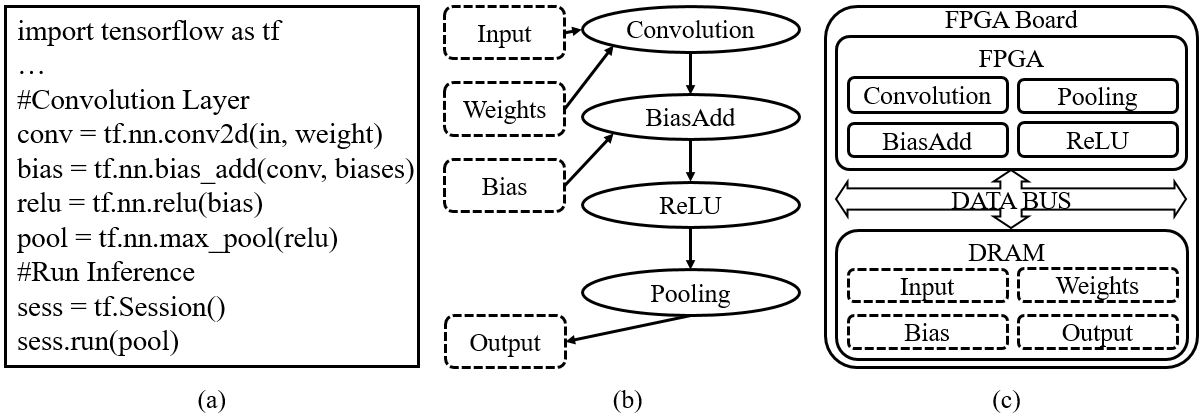
\includegraphics[width=1.0\linewidth]{./figure/tf.jpg}
	\caption{Comparison between TensorFlow and FPGA Implementation}
	\label{tf}
\end{figure}

\subsection{OpenCL-based HLS}
It is well-known that using hardware description languages (e.g. Verilog, VHDL) to design FPGAs is quite hard and time-consuming. Besides, the learning curve for beginners in hardware development is very steep. These two reasons make hardware design a heavy work for researchers. Fortunately, high-level-synthesis (HLS) tools help us solve this difficult problem. These tools receive designs programmed by high-level programming languages (C, C++, OpenCL, etc.), then transform them into the corresponding HDL descriptions and get the the final hardware configuration files. Among these tools, OpenCL-based HLS tool wins great popularity due to its flexible framework and great portability. Figure \ref{OpenCL-HLS} shows a rough framework of the FPGA implementations designed by OpenCL-based HLS. Similar to other OpenCL-based frameworks, the whole system is comprised of two main parts: $Host$ and $Device$. $Host$ is a desktop computer or server, where a C/C++ program is compiled and executed to perform the controlling operations. $Device$ is an FPGA board, which is plugged into the motherboard of $Host$ through a PCI-e slot. Data communication between $Host$ and $Device$c are accomplished through this PCI-e slot, and this slot is also used to power and program FPGA. Inside FPGA, hardware modules are compiled and invoked by $Host$ to complete the main computation tasks.

\begin{figure}
\centering
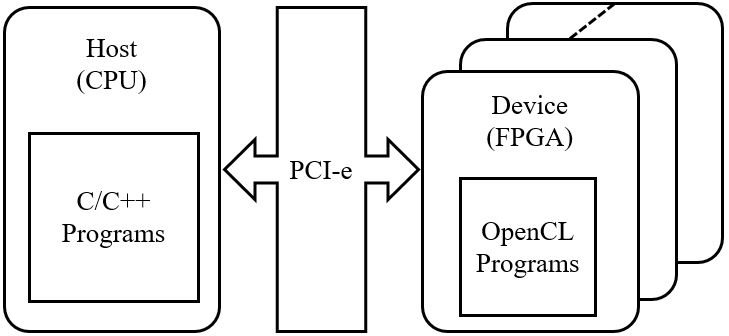
\includegraphics[width=1.0\linewidth]{./figure/OpenCL-HLS.jpg}
\caption{OpenCL-HLS Framework}
\label{OpenCL-HLS}
\end{figure}


\section{Framework}
We introduce the architecture of our proposed framework in this section. We first give an overview, then discuss about the main parts of it separately.

\subsection{Overview}
An overview of our overall framework is shown in Figure \ref{framework}.The whole framework is mainly comprised of two parts: $Symbolic\ Compiler$ and $Accelerator$. Symbolic descriptions (TensorFlow in our case) of deep learning models are fed into $Symbolic\ Compiler$, which generates the programs to be executed on $Host$ and the binary files to program FPGA. $Accelerator$ performs the model inference in FPGA chip, and an on-board DDR3 DRAM works as the global memory for data storage. The whole framework works in an ``end-to-end'' manner: from software-based model descriptions (TensorFlow codes) to FPGA-based model inference implementations (FPGA programming files), and this procedure is all done automatically without any human intervention.

\begin{figure}
	\centering
	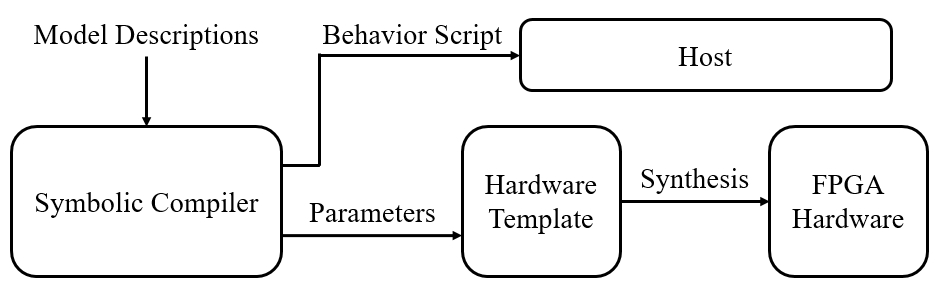
\includegraphics[width=1.0\linewidth]{./figure/framework.jpg}
	\caption{Overall Framework}
	\label{framework}
\end{figure}

\subsection{Symbolic Compiler}
TensorFlow has provided many useful APIs for deep learning researchers. All these functions can be regarded as computation nodes which constitute the final computation graph. As a result, our $Symbolic\ Compiler$ also starts from the function level of TensorFlow for simplicity and intuition. For now, our $Symbolic\ Compiler$ can support about XX \% of the functions or APIs that are related to deep learning model inference provided by TensorFlow.

The detailed structure and working flow of our $Symbolic\ Compiler$ are shown in Figure \ref{sc}. First, we design a $U.S.E.\ Compiler$ to convert TensorFlow described deep learning models into a Unified Symbolic Expression (U.S.E.). U.S.E. describes the topological structure and functionality of the models to be deployed, such as: layer numbers, layer types, input/output sizes, etc. The $U.S.E.\ Compiler$ is a compiler based on LLVM [cite], which can analyse the function-level computation graph inside programs through arguments dependency. The U.S.E. file is then fed into a $Analyser$ to decide the optimal hardware configurations with the help of some performance and resource models. $Code\ Generator$ uses these chosen parameters to generate the corresponding OpenCL codes for both $Host$ and $Device$. After that, we use Altera AOCL tools to synthesis and compile the generated OpenCL codes for $Device$, and get the final binary files to program FPGA.  

\begin{figure}
	\centering
	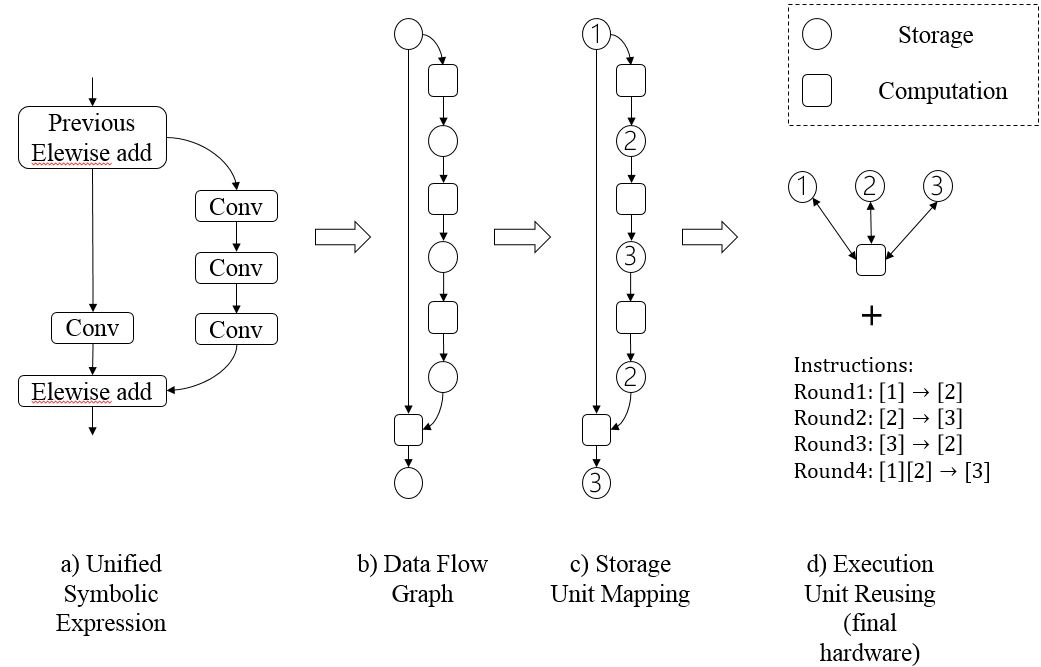
\includegraphics[width=1.0\linewidth]{./figure/sc.jpg}
	\caption{Symbolic Compiler}
	\label{sc}
\end{figure}

%We use open-source codes analyzing tools (e.g. Clang, llvm?) to analyze the topological structure of computation graph, then we translate it into U.S.E with a little modifications. Since our framework is designed for implementing inference phase of deep learning models, we define ``Layer'' as the basic block of U.S.E.. If and only if a new set of parameters (weights and bias) is fed into the model, a new Layer begins. This means that a single Layer in U.S.E. may consists of several stacked functions (computation nodes) in TensorFlow, but only a single W and B input. In Codes \ref{use}, the left shows an pseudo-code of a simple model description in TensorFlow (little requirements), and the right is the corresponding U.S.E. generated by our Compiler. 


\subsection{Accelerator}
$Accelerator$ is the main part of our hardware implementation for model inference. However, the massive options for model structures bring great difficulty for hardware implementations of deep learning models. To support various types of deep learning models in our framework, a unified computation kernel is strongly demanded. We find that deep learning models are always constructed by stacking layers, and the main computation inside each layer is or can be converted to matrix multiplication. As a result, we implement an efficient matrix multiplication (MM) kernel to perform model inference, instead of implementing each layer or model individually. To insure the model functionality and correctness, we add data management kernels to cooperate with the MM kernel.

$Accelerator$ is mainly comprised of three OpenCL kernels: $MM$, $Data_{in}$and $Data_{out}$. $MM$ performs matrix multiplication, and details about it are provided in Section 4.1. $Data_{in}$ and $Data_{out}$ are data management kernels that convert input or output data into the format required by $MM$. All these kernels work in a single-work item mode, which offers great convenience to our design and code generating. The optimization parameters and resource utilization can be compile-time reconfigurable, which provides possibilities for $Symbolic\ Compiler$ to choose the optimal design configuration.

Since the computation and data accessing pattern vary among different types of deep learning models, the strategies for converting them into MM are also quite different. So details about the converting methods in $Data_{in}$ and $Data_{out}$ for typical types of layers are provided as follows. 

\subsubsection{Fully-Connected Layers}
The computation performed in fully-connected layers can be summarized as Equation \ref{fc}. These layers output a vector ($Out$) as the multiplication of input vector ($In$) and weight matrix ($Weight$). The corresponding API in TensorFlow for fully-connected layers is $tesorflow.matmul()$.

\begin{equation}
\centering
Out[x]=\sum_{i=1}^{N_i}In[i]\ *\ Weight[x][i]
\label{fc}
\end{equation}

As a result, computation inside fully-connected layers can be viewed as matrix multiplying vector. Thus, we can use our $MM$ kernel to perform it by simply setting one dimension of input matrix to 1. 

\subsubsection{Convolution Layers}
The computation performed in convolution layers can be summarized as Equation \ref{conv}. These layers take a set of feature maps as input, and convolve these input with all the trained weights, then output a set of extracted feature maps. The corresponding API in TensorFlow for convolution layers is $tensorflow.nn.conv2d()$.

\begin{equation}
\centering
Out[x][y][z]=\sum_{i=1}^{N_i}\sum_{j=1}^{K}\sum_{k=1}^{K}In[i][y+i][z+k]*W[x][i][j][k]
\label{conv}
\end{equation}

To use the $MM$ kernel for the convolution layers, we need to convert the convolution operations into matrix multiplication, and the general strategy for converting a 2d-convolution into MM is provided in Figure \ref{convert}. In this example, there are $M$ input feature maps and $N$ output feature maps. The size of each output feature map is $R\times C$. The size of convolution kernels is $K\times K$, and the sliding stride of convolution is $S$. Here is how we do the converting: First, we partition each output feature map into a single column of the output matrix. To calculate one pixel of one output feature map, we need a patch of input features (size of $K\times K\times M$) and a set of convolution kernels (size of $K\times K\times M$), so we partition a patch of input into a single row of input matrix and the corresponding set of convolution kernels into a single column of weight matrix. All these converting work and data address computing are done in $Data_{in}$ and $Data_{out}$. Once the converting work is done,  we can use our $MM$ kernel to perform convolutions.

\begin{figure}
	\centering
	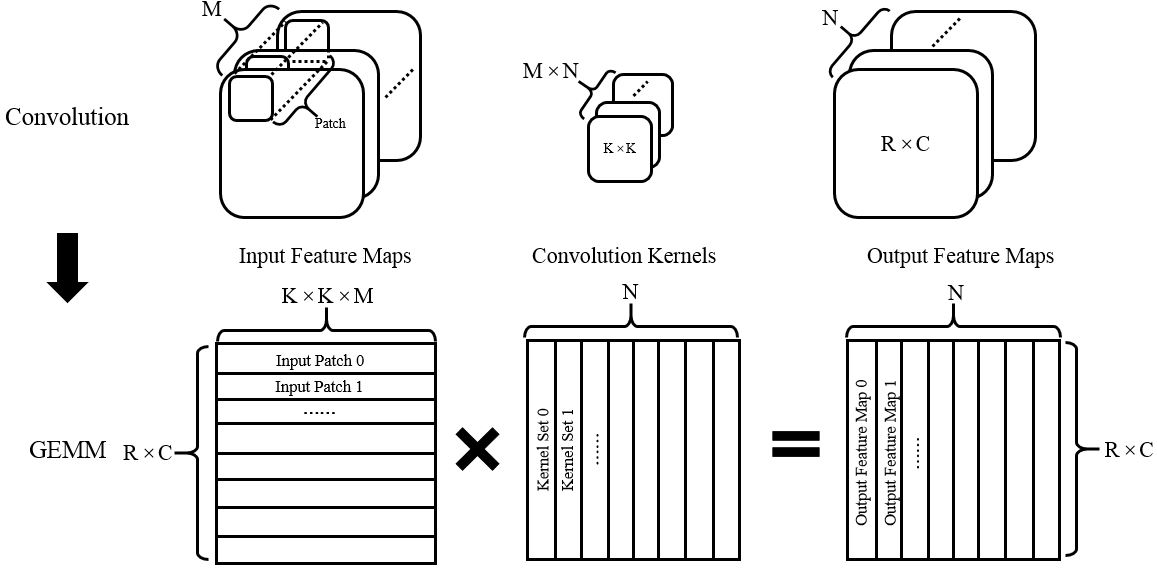
\includegraphics[width=1.0\linewidth]{./figure/convert.jpg}
	\caption{Convert}
	\label{convert}
\end{figure}

\subsubsection{Recurrent Layers}
For basic recurrent layers, the computation inside them is the same as fully-connected layers, which has already been discussed about in Section 3.3.1. While in recent years, Long Short-Term Memory (LSTM) has gained great popularity in RNN design. These LSTM-RNNs use LSTM cells in their topological structure, and achieve state-of-the-art performance in several applications. There is also a corresponding API in TensorFlow for LSTM-RNN, $tensorflow.rnn_cell.BasicLSTMCell()$. Numerous variants of LSTM structures have been proposed, while xx et.al claim that all these variants show little difference in model accuracy []. So we implement the LSTM cell described in Equation \ref{lstm0} to \ref{lstm4}, which is also the implementation in TensorFlow API.

\begin{equation}
\centering
G_i[x]=\sigma(\sum_{i=1}^{N_i}In[i]*W_ii[x][i]+\sum_{j=1}^{N_h}H[j]*W_ih[x][j])
\label{lstm0}
\end{equation}
\begin{equation}
\centering
G_f[x]=\sigma(\sum_{i=1}^{N_i}In[i]*W_fi[x][i]+\sum_{j=1}^{N_h}H[j]*W_fh[x][j])
\label{lstm1}
\end{equation}
\begin{equation}
\centering
G_c[x]=tanh(\sum_{i=1}^{N_i}In[i]*W_ci[x][i]+\sum_{j=1}^{N_h}H[j]*W_ch[x][j])
\label{lstm2}
\end{equation}
\begin{equation}
\centering
G_o[x]=\sigma(\sum_{i=1}^{N_i}In[i]*W_fo[x][i]+\sum_{j=1}^{N_h}H[j]*W_fo[x][j])
\label{lstm3}
\end{equation}
\begin{equation}
\centering
Out[x]=G_o[x]*tanh(G_f[x]*Cell[x]+G_i[x]*G_c[x])
\label{lstm4}
\end{equation}

Equation \ref{lstm0} to \ref{lstm4} show that the main computation inside LSTM-based recurrent layers is still matrix multiplying vector. As a result, we apply similar conversion to that of fully-connected layers, and add extra data buffers and controlling units to insure the functionality is correct.

\subsubsection{Pooling Layers}
Typically, pooling layers take the maximum (max-pooling) or the average (average-pooling) of the input features in a pooling window as the result to output. The corresponding API in TensorFlow is $tensorflow.nn.max_pool()$ and $tensorflow.nn.avg_pool()$. Pooling layers are always responsible for sub-sampling features, and not much computation is involved in them. As a result, if the target model includes pooling layers, we will add additional kernel to perform it instead of converting it into MM. 

\subsubsection{Activation Layers}
The operations in activation layers are always element-wise functions to the features, so there is no need to implement an extra kernel for it or convert it into MM. We simply add them to $Data_{out}$ before the outputs are written backc. However, there are several types of activation functions. For simpler ones like ReLU ($tensorflow.nn.relu()$ in TensorFlow), we implement them directly as they are. For ones including complex exponential operations like tanh ($tensorflow.tanh()$ in TensorFlow) and sigmoid ($tensorflow.sigmoid()$ in TensorFlow), we use linear approximation [cite] to further improve performance and resource utilization, which is also a common optimization for hardware implementation [cite]. The experiments show that the accuracy loss is XX\%, which is small enough to be ignored.

\section{Implementation  Details}
In this section, we introduce the details of our hardware implementation, and propose a model to estimate the overall performance of our design.

\subsection{MM Kernel}
Since the size of matrices during deep learning model inference is usually too large to be processed all at once with the limited on-chip resource, we propose to perform these calculations in a tiling style, which is also the task of $MM$. Another advantage that the tiling strategy can bring is we can better explore the data locality, and improve the whole efficiency of matrices multiplication. Our tiling strategy can be generally shown in Figure \ref{tile}. The output matrix is tiled both in row and column, and the tiling size is denoted as $S_{tile}$. Then the two input matrices are tiled correspondingly to accomplish the matrix multiplication. To insure the computation are correctly performed in a tiling manner, we apply zero-padding to input matrices if any dimension of them is not divisible by its tiling size.

%\begin{figure}
%	\centering
%	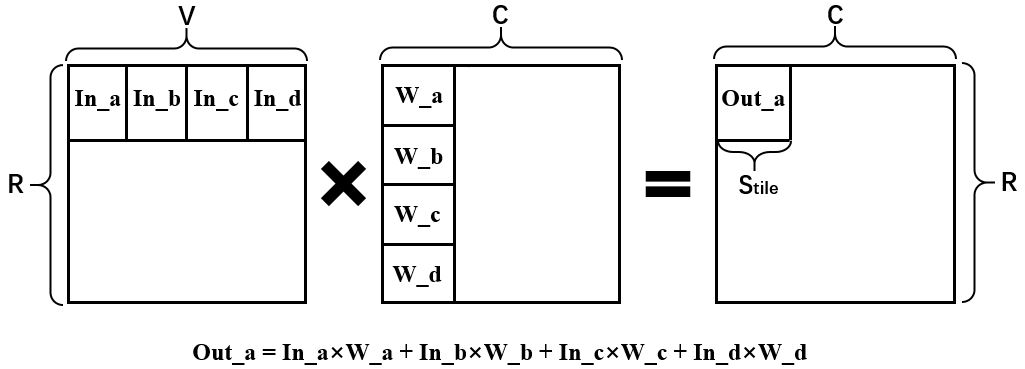
\includegraphics[height=2in, width=3in]{./figure/tile.jpg}
%	\caption{Tiling}
%	\label{tile}
%\end{figure}
\begin{figure}[h]
	\centering
	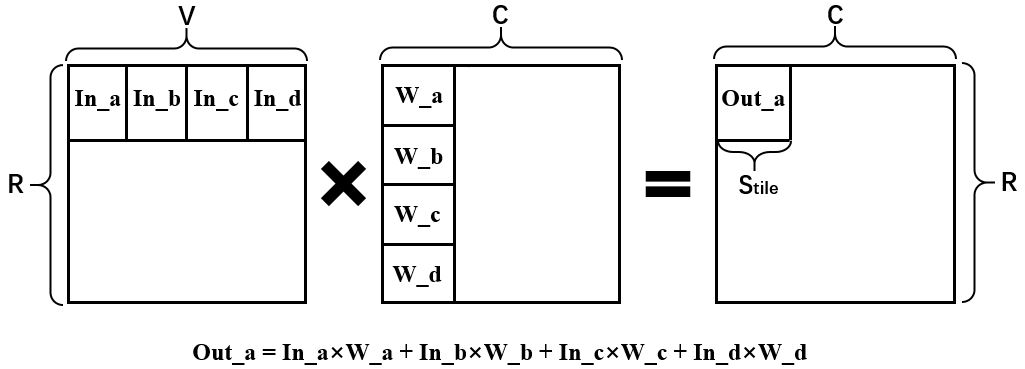
\includegraphics[width=1.0\linewidth]{figure/tile.jpg}
	\caption{Tiling}
	\label{tile}
\end{figure}

Figure \ref{mm} shows the detailed structure inside $MM$. $MM$ takes in two tiles of input matrices, and performs the tiled matrix multiplication in $Dot\ Product\ Unit$ vector by vector. All the input data are fed into multipliers simultaneously, then the temporary results are summed up through a reduction tree to minimize the computing latency. Once $MM$ gets a final result, it sends it out through a data channel.  

Besides, we implement two on-chip buffers ($Buffer0$ and $Buffer1$ in Figure \ref{mm}) using two deep FIFOs. These two buffers are used to buffer the tiled input data, and they operate in a ping-pong manner: During a certain phase, $Dot\ Product\ Unit$ is processing with the tiles fetched from $Buffer0$, and the tiles to be processed in the next phase are loaded into $Buffer1$ simultaneously. Once $Dot\ Product\ Unit$ finished computing with current tiles, it comes to the next phase, and every operation reverses. $Dot\ Product\ Unit$ processes the tiles fetched from $Buffer1$, and $Buffer0$ loads the next tiles. In this manner, $MM$ can overlap data communication with computation in time dimension, and significantly improve the throughput of $MM$.

\begin{figure}
	\centering
	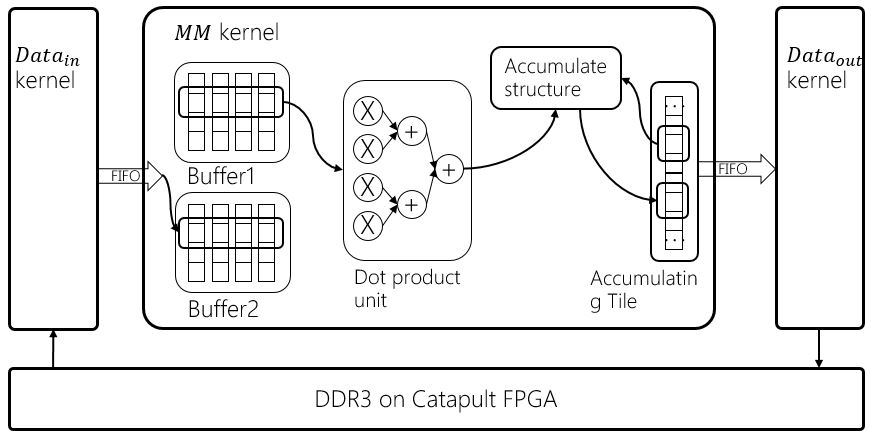
\includegraphics[width=1.0\linewidth]{./figure/tree.jpg}
	\caption{MM kernel}
	\label{mm}
\end{figure}

Numerous prior works have shown that deep learning models are robust enough even with a decrease on data precision. Many great works [cite, cite,...] on accelerating deep learning model inference used fixed-point parameters in their design for performance improving and resource saving. Recently, Bengio et.al found that deep CNN models can even use binary values for model inference without much accuracy loss[cite]. So in our implementation, we also support implementing a fixed-point version of the target model. Designers using our framework can enable it by simply adding a ``$-fixed\_point$'' compilation option to our $Symbolic\ Compiler$. However, the accuracy loss brought by data quantization must be estimated and tested by the model designers in advance, and they need to make a decision on the trade-off between accuracy and performance. 

\subsection{Data Layout Optimization}
As introduced in Section 3.3, we convert different types of layers into $MM$. The correctness and effectiveness are guaranteed by carefully designed data fetching strategies. However, these data fetching schemes usually need extra operations for address translation, and usually behaves random DRAM accessing, which bring great overhead on data fetching and storing. As a result, we propose to solve this tricky problem by optimizing data layout.

Here we use a simple example to illustrate the problem and our corresponding optimization. According to Section 3.3, convolution layer performs the most complex convention and data reshaping operations, so we take it for explanation in Figure \ref{datalayout}. We denote the number of input feature maps and size of convolution kernel as $N_{fmap}$ and $K\times K$ respectively. As shown in Figure \ref{datalayout}, we set $N_{fmap}=64$ and $K=2$ in our example. The size of input feature map is 3$\times$3, and the sliding stride of convolution kernel is 1. Conventionally, all input feature maps are stored in DRAM in row-major manner, the detailed storage status is shown in Figure\ref{conventional}. According to Section 3.3 and Section 4.1, we convert the convolution in to matrix multiplication, and perform it in a tiled manner. Here we set the tiling size $S_{tile}=8$. Prior work [cite] usually take advantage of on-line address computing to fetch the proper data for $MM$. Thus, in each row within a tile, there are 8 ($S_{tile}[2][K\times K]$) input features. For the first layer, we illustrate the corresponding DRAM accessing pattern in Figure \ref{conventional}. Unfortunately, this random reading pattern requires recharge for DRAM. Along with the extra address converting computation, the actual bandwidth between DRAM and FPGA chip is restricted to xx GB/s, which makes I/O a critical bottleneck of the overall performance.

\begin{figure}
	\centering
	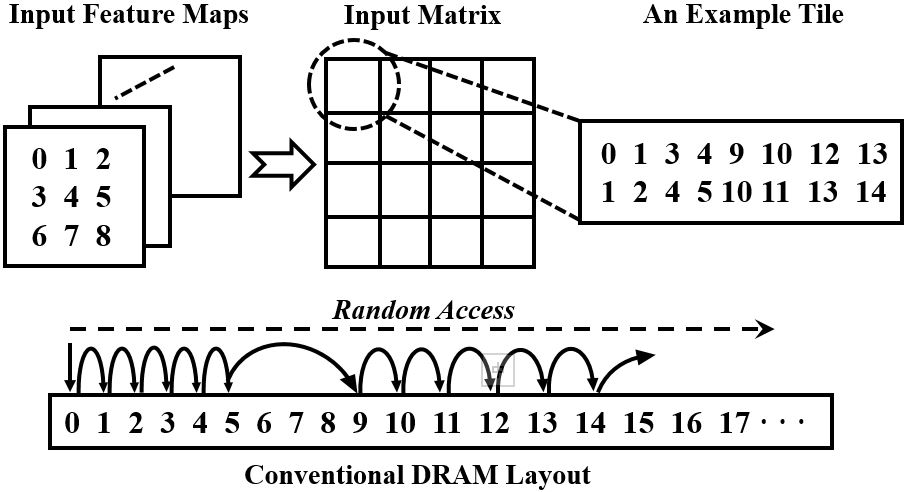
\includegraphics[width=1.0\linewidth]{./figure/conventional.jpg}
	\caption{conventional}
	\label{conventional}
\end{figure}

\begin{figure}
	\centering
	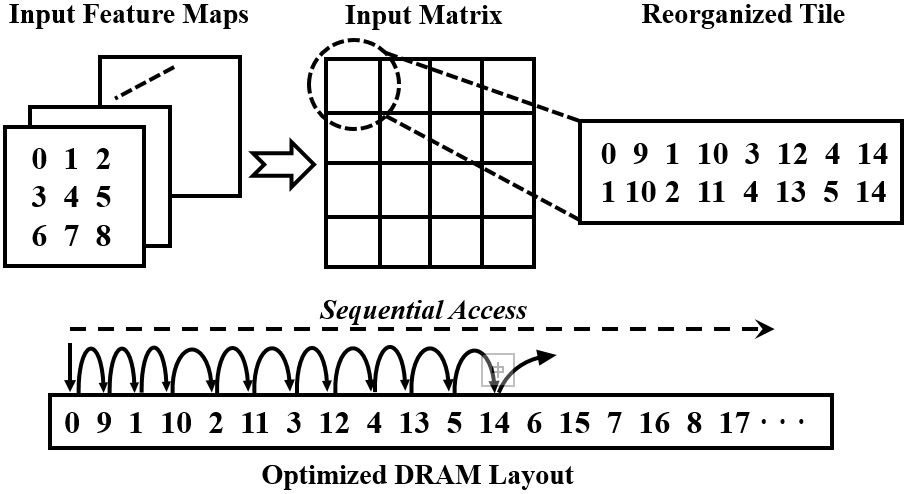
\includegraphics[width=1.0\linewidth]{./figure/layout.jpg}
	\caption{layout}
	\label{datalayout}
\end{figure}

To issue this problem, we optimize the data layout of input feature maps. The result after data layout optimization is generally shown in Figure \ref{datalayout}. For each row within a tile, we reorganize the input features from $S_{tile}[2][K\times K]$ to $S_{tile}[K\times K][2]$. In other words, we packed the features at the same position of each feature map together, and store them in DRAM together to fit the characteristics of sliding convolution kernel. The corresponding DRAM storing status is also shown in Figure \ref{datalayout}. The other input matrix, weight matrix, need to be adjusted accordingly, but the overhead brought by this can be ignored since weights are pre-trained and these adjustments can be applied before model deployment. Thus, with the optimized data layout, the data accessing pattern is in a sequential way, which improves the bandwidth between DRAM and FPGA chip to xx GB/s, and optimizes the bandwidth constraint greatly.  

For other layers, like fully-connected layers and recurrent layers, the 
optimization strategies are similar. We can regard them as convolution layers whose $K=1$, and all the layers can share the same data layout optimization strategies.

\subsection{Performance Estimation}
Before finally deploying deep learning models onto FPGA, model designers may want to have a rough estimation about the performance for model inference. The estimated results are also quite helpful for model designers to improve their designs. As a result, our framework can report an estimated performance of the target deep learning model on FPGA.  

The total number of operations inside a $MM$ kernel can be estimated as  $2\times S_{tile}^3$. The execution time of a $MM$ includes both matrix multiplication and data communication, so the total cycles used for a tile is $S_{tile}^3 \div N_{DSP}$(???).
As a result, we can estimate the performance (in GOPS, giga operations per second)of our $MM$ kernel through Equation \ref{perf}, where $Freq$ indicates the running frequency of FPGA board.

\begin{equation}
\centering
\begin{split}
Performance\ &=\ \dfrac{Operations}{Execution\ Time} \\
&=\ \dfrac{2\times S_{tile}^3}{Cycles/Freq}
\end{split}
\label{perf} 
\end{equation}

Equation \ref{perf} shows that several parameters ($S_{tile}$, $N_{DSP}$,..) can vary in different implementations. Each group of choices for these parameters corresponds to a possible configuration for hardware implementation. Thus, the massive possibilities form a huge design space. So we need to explore the whole design space for the optimal one. This exploration problem can be formulated as follows.
\begin{equation}
\centering
\begin{split}
&Variable:\ Optimization\ parameters???, Frequency \\
&Constraints: Resource (DSP), Bandwidth \\
&Target: Maximum Performance((areto\ Optimality)
\end{split}
\end{equation}
 
This exploration work can be accomplished by simple algorithms for integer programming problems. The $Symbolic\ Compiler$ in our framework can help to explore the design space and  find the optimal hardware configuration. Then it will report the estimated performance and generate the corresponding codes for HLS tools.

\section{Evaluation}
To illustrate the effectiveness and great performance achieved by our proposed framework, we design and implement three models as our case studies for modern typical deep learning structures: ANN (or feedforward neural network), CNN, and RNN. 


\subsection{Experimental setup}
For the software part, the $Symbolic\ Compiler$ that performs performance estimation, resourse estimation, parameter decision, and OpenCL codes generation is written in Python X.X. To implement our desing on FPGA board, we take advantage of a high-level synthesis design tool, AOCL (vXXX). This high-level synthesis tool help us synthesis and implement the OpenCL-based codes into binary files to program FPGA. The codes on host is written in C++, and compiled by Visual Studio XXX.

For the hardware part, we use a PikesPeak FPGA board, with an Altera XXXX chip on it. An 8GB DDR3 is integrated with the FPGA chip as external storage. The working  frequency of the whole hardware implementation is set to 200MHz. This FPGA board is plugged into a PCI-e slot of a host PC. The CPU inside host is XXXXX, XXGHz,

For performance comparison, we implement software inference on a Xeon CPU, the working frequency of it is xx GHz, with a XXMB Cache.

\subsection{Experimental results}

\subsubsection{Performance}
$MM$ kernel is the core part of FPGA-based model inference, so we compared the performance of our $MM$ kernel with that of Intel MKL and Altera example design in Figure \ref{performance}. We have two versions of implementations: floating-point (32 bits) and fixed-point (8 bits).
MM performance , comparison with Intel MKL and Altera Example Design, floating and fixed
\begin{figure}
	\centering
	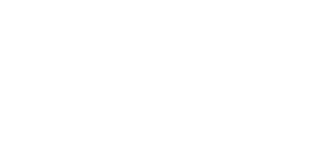
\includegraphics[width=1.0\linewidth]{./figure/blank.jpg}
	\caption{performance}
	\label{performance}
\end{figure}

To show the performance for whole model. we take CNN inference as an example, since there have been massive prior work on it. the comparison results are shown in Table \ref{cnn}
\begin{figure}
	\centering
	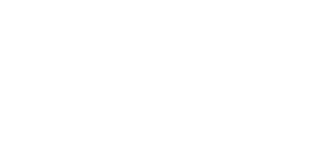
\includegraphics[width=1.0\linewidth]{./figure/blank.jpg}
	\caption{performance}
	\label{cnn}
\end{figure}

\subsubsection{Energy Efficiency}
energy efficiency compared with Xeon CPU, multi benchmarks:ANN, CNN, RNN, LSTM...

\begin{figure}
	\centering
	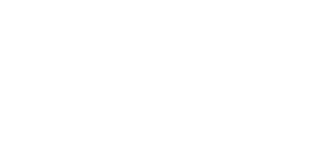
\includegraphics[width=1.0\linewidth]{./figure/blank.jpg}
	\caption{performance}
	\label{ee}
\end{figure}

\subsubsection{Framework Effectiveness}

design time, modelling accuracy

First, we discuss about the great improvement on designing efficiency achieved by our proposed framework. For all the three case studies in this section, our framework meanly takes about 4-5 hours to accomplish the hardware implementation from TensorFlow-described models. While it will take a experienced hardware engineer two weeks to implement one deep learning model on FPGA. So our framework can improve the efficiency of deep learning models' deployment by about 80x. Furthermore, designers with little knowledge about hardware implementation details can also easily use our framework, which indicates that our framework can be widely popularized and benefit the FPGA community.

estimated and tested?

%\section{Related work}

\section{Conclusions and future work}
In this paper, we propose a framework that automatically migrates TensorFlow described deep learning models to FPGA implementation for inference acceleration. We also propose several performance models and resource estimations to choose the optimal design configuration. Our case studies show the great performance and effectiveness achieved by this framework.

However, there are still several directions for future research. First, we will go on working with a distributed version of this framework on an FPGA fabric. Second, we will adapt the kernels inside our framework to support emerging optimization techniques for deep learning models like pruning, binarization, etc. Last but not least, we will further extend our framework to model training.


%ACKNOWLEDGMENTS are optional
%\section{Acknowledgments}

%
% The following two commands are all you need in the
% initial runs of your .tex file to
% produce the bibliography for the citations in your paper.
\bibliographystyle{abbrv}
\bibliography{sigproc}  % sigproc.bib is the name of the Bibliography in this case
% You must have a proper ".bib" file
%  and remember to run:
% latex bibtex latex latex
% to resolve all references
%
% ACM needs 'a single self-contained file'!
%

% That's all folks!
\end{document}
